\label{sec:bg}
%Rails applications are structured based on the model-view-controller
%(MVC) architecture. We illustrate this architecture in Figure~\ref{fig:ormf}. When a client requests for a URL such as {\tt http://foo.com/projects/index/1} \alvin{to make it more real how about change ... to something like foo.com}, Rails maps these requests to the controller action as shown in the Routing rules as shown in the figure \alvin{what does these rules do? is it important to know about them in this paper?}.  The mapped \alvin{?} Controller takes in the parameters from the requests and asks model to retrieve data from database. The returned data then is used to generate view which will be sent to the client side. An action is a member method of a Ruby controller class. There could exist multiple actions in a controller file to handle  different user requests. \alvin{the description here needs to map to the figure. I suggest taking a look at the description in our CIKM paper or the ICSE paper}\cong{I'll revise it.}
\iffalse 
\begin{figure}[ht]
    \centering
    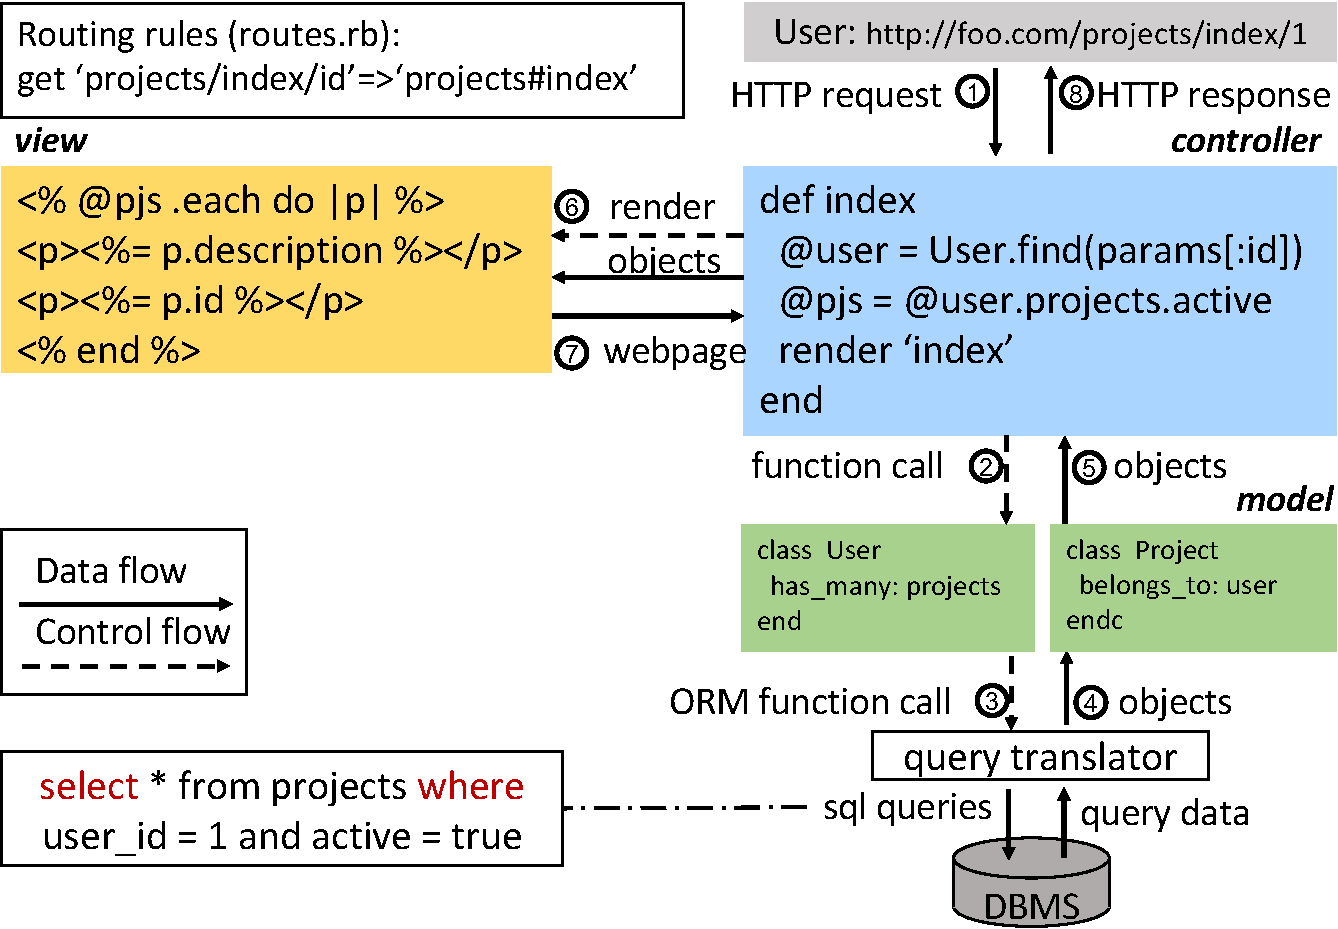
\includegraphics[width=1\columnwidth]{figs/ormf.pdf}
    \vspace{0.05in}
    \caption{Rails application architecture }
    \label{fig:ormf}
    \vspace{-0.2in}
\end{figure}
\fi 

% \subsection{Architecture of web applications} 
% % Rails applications are structured based on the model-view-controller (MVC) architecture. When a client requests for a URL such as {\tt http://foo.com/projects/index/1}, a {\it controller} action ``{\tt projects /index}'' is triggered. This action takes in the parameters from the request (e.g., ``{\tt 1}'' in the URL as {\tt params[:id]}) and interacts with the DBMS by calling the ActiveRecord API implemented by the Rails Object-Relational Mapping (ORM) framework. Rails translates the function calls into SQL queries, whose results are serialized into {\it model} objects (e.g., the {\tt Project} model) and returned to the controller. Then, the returned objects are passed to the {\it view} files to generate a webpage to send back to users. Each model is derived from {\tt ActiveRecord}, and is mapped to a database table by Rails. 
% Applications built using the Ruby on Rails framework are structured using the model-view-controller (MVC) architecture. 
% For example, when a web user submit a form through a URL like {\tt http://foo.com/wikis/new/title=release}, a {\it controller} action ``{\tt wikis/create}'' is triggered. This action takes in the parameters from the request (e.g., ``{\tt release}'' in the URL as {\tt params[:title]}) and interacts with the database by calling the ActiveRecord API implemented by the Rails Object-Relational Mapping (ORM) framework. Rails translates ActiveRecord function calls into SQL queries (a write query in this case), whose results are then serialized into {\it model} objects (e.g., the {\tt Wiki} model) and returned to the controller. The returned objects are then passed to the {\it view} files to generate a webpage that is sent back to users. Each model is derived from {\tt ActiveRecord}, and is mapped to a database table by Rails. 
% %The data retrieval is done by translating a {\tt ActiveRecord} API call into a database query. The returned database tuples are converted into objects and sent to a {\it view} be rendered. 
% A view file (ends with {\tt .erb} or {\tt .haml}) usually involves multiple languages including HTML, JavaScript, and Ruby. 
% %The ruby code can dynamically decide which element to show. 

\subsection{Constraints in web applications}
\label{sec:back_constraints}



%\shan{this sub-section might better belongs to the background or we can have a taxonomy section or something like that} 

We roughly categorize data constraints into three types based on where they are checked and specified
as shown in Table~\ref{table:constraintdeftax}.

%\shan{XXX what exactly is the definition of ``different layers''? Is it based on where the checking is conducted?}

\textbf{Front-end constraints.} 
Developers can use regular expressions to specify constraints
about a particular HTML data-field inside a view file, such as the {\tt pattern=`.+'} for the {\tt title}
field %in {\tt views/wiki/new.html.erb} 
in Figure~\ref{fig:crossstack}. The majority of such constraints are related to persistent data maintained by the database.
 
Such constraints are checked when the user submits a web form. Failure to validate will cause the form submission to fail, with an error message specified by developers shown next to the corresponding HTML field, with all the previously filled contents remain on the page.
%with other filled contents on the page. \alvin{seems a bit too detail? maybe just say `Failure to validate will cause the form submission to fail with an error shown on the page'?}

%\shan{other the already filled content on the page will still be there, right? XXX}.
  %\shan{according to your figure, the error message should be ``invalid title'', right? XXX}. 
%\utsav{We are only considering standard HTML constraints (e.g. min/maxlength, pattern, etc.), and we might want to investigate how frequently constraints are instead expressed as ruby code in the view layer, which I think may be possible in templates. } \junwen{TODO: collect the stats about the if checking in the view file in the non-API constraints}

\textbf{Application constraints.} 
Rails developers use {\it validation functions} to specify constraints of data fields in model classes.
Similar mechanisms exist in other ORM frameworks, such as validator functions in Django \cite{django-annotation}, and validator annotations in Hibernate \cite{hibernate-annotation}.

\begin{table}
\centering
\setlength{\tabcolsep}{1.2pt}  
\caption{Different types of constraints in web apps}
\label{table:constraintdeftax}
\resizebox{.7\columnwidth}{!}{
\begin{tabular}{@{}llll@{}}
\toprule
{\bf Run-time check}               & {\bf Source-code} & {\bf Specification}  & {\bf Specification} \\ 
{\bf location}                     & {\bf location}    & {\bf language}       & {\bf API} \\
\midrule
Front end                          & View  & HTML & Reg. expression           \\ \midrule
\multirow{3}{*}{Application server}& Model & Ruby & Built-in validation API    \\ \cmidrule(l){2-4} 
                                   & Model & Ruby & Custom validation API  \\ \cmidrule(l){2-4} 
                                   & Model/Controller&Ruby & Custom sanity check \\ \midrule
\multirow{2}{*}{Database server}   & Migration files &Ruby& ActiveRecord::Migration API\\ \cmidrule(l){2-4} 
                                   & Migration files &SQL & SQL ALTER TABLE queries   \\ \bottomrule
\end{tabular}
}
 \vspace{-0.2in}
   
\end{table}

% hibernate: https://hibernate.org/validator/documentation/getting-started/
% django: https://docs.djangoproject.com/en/2.2/ref/validators/

A validation function is automatically triggered every time when the application saves an object of the corresponding model class (i.e., when the ORM framework saves the corresponding record into the database).
Validation failure will cause the corresponding form to fail. The error message associated with the validation function will be shown to web users if developers put error checking and error-message display code in the view file.
%, as shown in Figure \ref{fig:error-msg}. 
%TODO. will add back the figure if we have space

\iffalse 
\begin{figure} 
    \centering
    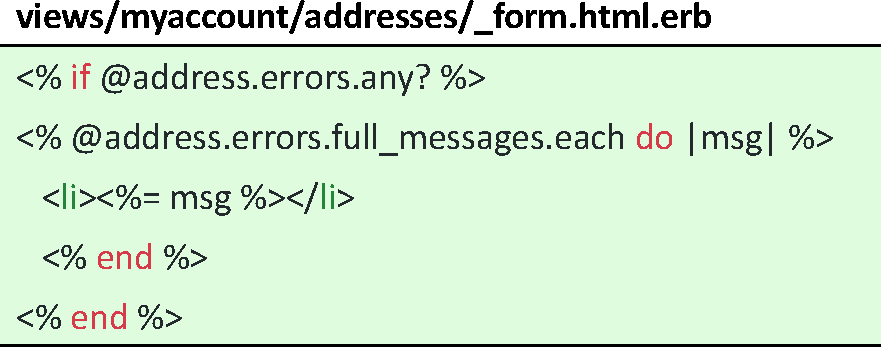
\includegraphics[width=0.9\columnwidth]{figs/error-messages-model.pdf}
    \caption{Error-message rendering in Ror-ecommerce \cite{ror}}
    \label{fig:error-msg}
    \vspace{-0.1in}
\end{figure}
\fi 

\iffalse 
\begin{figure} 
    \centering
    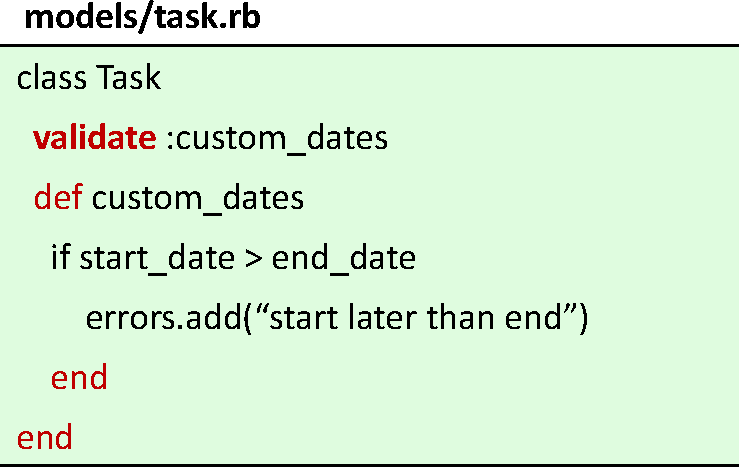
\includegraphics[width=0.7\columnwidth]{figs/custom-validator-example.pdf}
    \caption{Custom-validate code example}
    \label{fig:custom-validator-code}
\end{figure}
\fi  
 
Rails validation
functions include built-in ones, which cover many common constraints like text-field lengths (i.e., {\tt validates\_ length\_of}, as shown in Figure \ref{fig:crossstack}),
content uniqueness ({\tt validates\_ uniqueness\_of}), 
content presence ({\tt validates\_presence\_of}),
%numericality requirement ({\tt validates\_numericality\_of}),
as well as custom ones, where developers express more complicated constraints like keeping a strict order among multiple fields.
%as shown in Figure \ref{fig:custom-validator-code}.
%\utsav{Figure 3 needs to be fixed/reformatted..}

Developers can also constrain a data field through custom sanity checks, although they are uncommon in Rails. 
%These   checks typically are put right after a new set of inputs are obtained or right before saving content to database. 
%How to handle a sanity-check failure varies from case to case. 

 
%an order to the database, there will be a "if order.price > 0 " to restrict the price column of orders table is always greater than zero. 

\textbf{Database constraints.}  
Many data columns are associated with constraints inside the database (DB), like the {\tt varchar(30)} constraint shown in Figure \ref{fig:crossstack}. These constraints are specified in   the applications' migration files, which are used to alter database schema over time.
%xxx\shan{a one sentence definition of migration files?}. 
The majority of them (more than 99.5\%
in our studied applications) are specified through Rails Migration APIs, and are very rarely
specified through SQL queries directly (<30 cases
across all 12 applications we checked). 
%Once specified, they can be seen in the {\tt schema.rb} file in the Rails application. 
%\alvin{what does `can be seen in the rb file' mean? Is that file automatically generated?}\junwen{Yes, it can be generated through `rake db:migrate', which will create the final db schema through accumulating the migration files.}\shan{junwen, how about
%we remove the schema.rb sentence? we never use scheme.rb in the paper, right?}\junwen{sure}

These constraints are checked by the DB when an {\tt INSERT} or {\tt /UPDATE} query to the corresponding columns is issued (either by the application or DB administrator).
%sent either by the RAILs engine or directly by any people or program having access to the DB table.
If the check fails, the application will throw an {\tt ActiveRecord::StatementInvalid}
exception to indicate an underlying DB error. 
Unfortunately, in practice, developers almost {\it never} catch such exceptions
(it is caught in only 4 cases across thousands of model object saves 
across the 12 applications we studied). Hence, once triggered,
the web user's session will most likely crash, with all the filled-in contents lost with a cryptic SQL error shown to users. 
% \shan{how to specify
% error messages and how to display error messages for these cases?}

\textbf{Why are the constraints distributed across components?}
Front-end constraints are specified for web-form input data,
which is often related to DB record (e.g., used
as query parameters, compared with query results, etc.).  
Validation functions and DB constraints are specified only for
database fields, and are checked right before 
saving data into the DB.
The expressiveness of these two are similar --- most
constraints that are expressible using validation functions can also be written using
SQL queries or migration APIs, and vice versa.
Complicated constraints expressed using custom validation functions can   be expressed in the DB layer as
{\tt CONSTRAINT CHECK}s or custom stored procedures. However, neither layer can replace the other given the existence of ``backdoors,'' e.g., DB administrators updating data using the DB console, or sharing the same DB across multiple applications. Both are common practices~\cite{discourse-import}.

%\utsav{The Rails APIs allow users to specify nearly all types of constraints. The only cases where users must use custom SQL queries are: 1) adding custom "CHECK" constraints to DB (which allow users to limit domain of values, e.g. field > 0, or create customized multi-column constraints), 2) changing primary key constraints, or 3) performing changes to format that updates/casts existing data. However this custom SQL exists in the schema.rb file (and used infrequently - 4 cases).}\shan{?? what does it mean by having these SQL queries in scheme file?}


%%%%%%%%%%%%%%COMMONT OUT%%%%%%%%%%%%
%\shan{Junwen, please revise this paragraph.
%The example used here better to match an example that we will use later}

% \cong{junwen: can you change the figure, 1) reflect the data flow or the connection between MVC; 2) add the SQL query (since you estimate the SQL query time and how it contributes to a tag, I think it is important to add a concrete query in the example). 3) add circled number to the figure such that the text can easily refer, check CIKM figure2.}


% Rails maps each model class derived from {\tt ActiveRecord} to a single database table, for example a \textbf{User} class maps to the \textbf{users} table. The 
% {\tt ActiveRecord} interface also provides APIs that will be translated into
% database queries by ORM at run time.
% how the application responds to a specific web-page request. Inside
% an action there is code to retrieve database data through queries
% transparently translated by the ORM. Finally, the retrieved data is
% rendered via views that are often written in a template language, as
% shown in index.html.erb in Figure 1. Such views determine how
% the retrieved data is displayed in a client’s browser.
% The life cycle of a Rails application, and ORM applications in
% general, is as follows. When receiving a client HTTP request like
% “http://.../messages/index”, the application server first looks
% up the routing rules, shown at the top of Figure 1, to map this
% request to the index action inside MessagesController. When the
% index action executes, it invokes the @user.undeleted_messages
% function, which calls messages. where(...). The call to the Rails
% API where is dynamically translated to a SQL query by the Rails
% framework to retrieve data from the DBMS. The query results are
% then serialized into model objects and stored in @messages. The
% index action then calls render "index" to render the retrieved
% data in @messages using the index.html.erb template.



\iffalse
% \subsection{DB-aware static analysis of Ruby on Rails}
% \label{sec:back_adg}
% During preprocessing, previous work\cong{previous, or \Tool? if previous, which work?} inlines function calls to enable inter-procedural analysis later on. This
% process involves type inference \cite{furr2009static}% xxx \shan{how?}
% , as Ruby is dynamically typed \cite{an2009static}, and special
% handling to view files and filter functions. Specifically, 
% since view files may contain computation and queries too, 
% %\Tool identifies view files rendered by each controller and appends
% %Ruby code there to the controller action. 
% \Tool extracts the ruby code in each view and inlines them to the corresponding controller where the view is rendered.
% \Tool also inlines filter functions automatically invoked before an action
% and validation functions automatically invoked before every database-modifying function. 


% Previous work~\cite{powerstation} builds the PDG for an action through the intermediate representation(IR) compiled by JRuby~\cite{jruby}. Every node $n$ in the PDG represents a statement in the JRuby IR and 
% every edge $e$ represents either control dependency or data dependency. Furthermore, a data-dependency
% edge $n_1 \rightarrow n_2$ indicates that the output object $o$ of $n_1$ is used by $n_2$ without
% other statements overwriting $o$ in between. For each statement, we keep the line number information. Combining with the APIs provided by ActiveRecord and the database schema information, we further decide whether a node is a query. 

% The PDG generated above is then extended in three ways to create the ADG: 
% (1) changing and splitting some nodes to become 
% Query nodes; (2) annotating every Query node with the database table and fields that are read or written; 
% (3) annotating every outgoing data-dependency edge of a Query node with the exact field(s) that are used.

% To accomplish this, previous work first analyzes every model class that extends the Rails
% {\tt ActiveRecord} interface to determine all the database
% tables in the application and the association relationship among them.
% For example, analyzing the model classes illustrated in 
% Figure~\ref{fig:schema}, \Tool identifies the {\tt users} table
% corresponding to the {\tt User} class and similarly for the {\tt Blog} class, and that these two models have 
% a one-to-many relationship, i.e., each instance of {\tt User} may own multiple instances of {\tt Blog}.
% Second, \Tool analyzes the {\tt schema.rb} file to determine
% how many fields each table contains. For example, parsing the
% {\tt schema.rb} snippet in Figure~\ref{fig:schema}, \Tool learns about 
% the schemas of table {\tt users} and {\tt blogs} as
% shown in the bottom of the figure.

% Third, \Tool identifies queries from three sources: (1) explicit 
% invocations of
% Rails {\tt ActiveRecord} Query APIs, such as {\tt exist?},
% {\tt reload}, \textit{\tt update}, \textit{\tt destroy}, etc;
% (2) implicit queries generated by Rails to access object fields, e.g., {\tt $o_1$.$o_2$}, where 
% the class of $o_1$ and the class of $o_2$ are associated model classes
% (e.g., {\tt user.blogs} would incur a query to
% retrieve records in {\tt blogs} table that are associated with
% the specific {\tt user} record in {\tt users} table);
% (3) explicitly invoked raw SQL queries through  Base.connection.execute.
% %\junwen{it's also thru the ActiveRecord API, similar as the first type}
% Any query identified above is represented as a Query node in the ADG.\footnote{At run time,
% multiple such queries could be composed by ORM into one SQL query.
% Such query chaining does not affect \Tool analysis.} 

\fi